\section{Design Example}

\begin{figure}[tb]
\centering
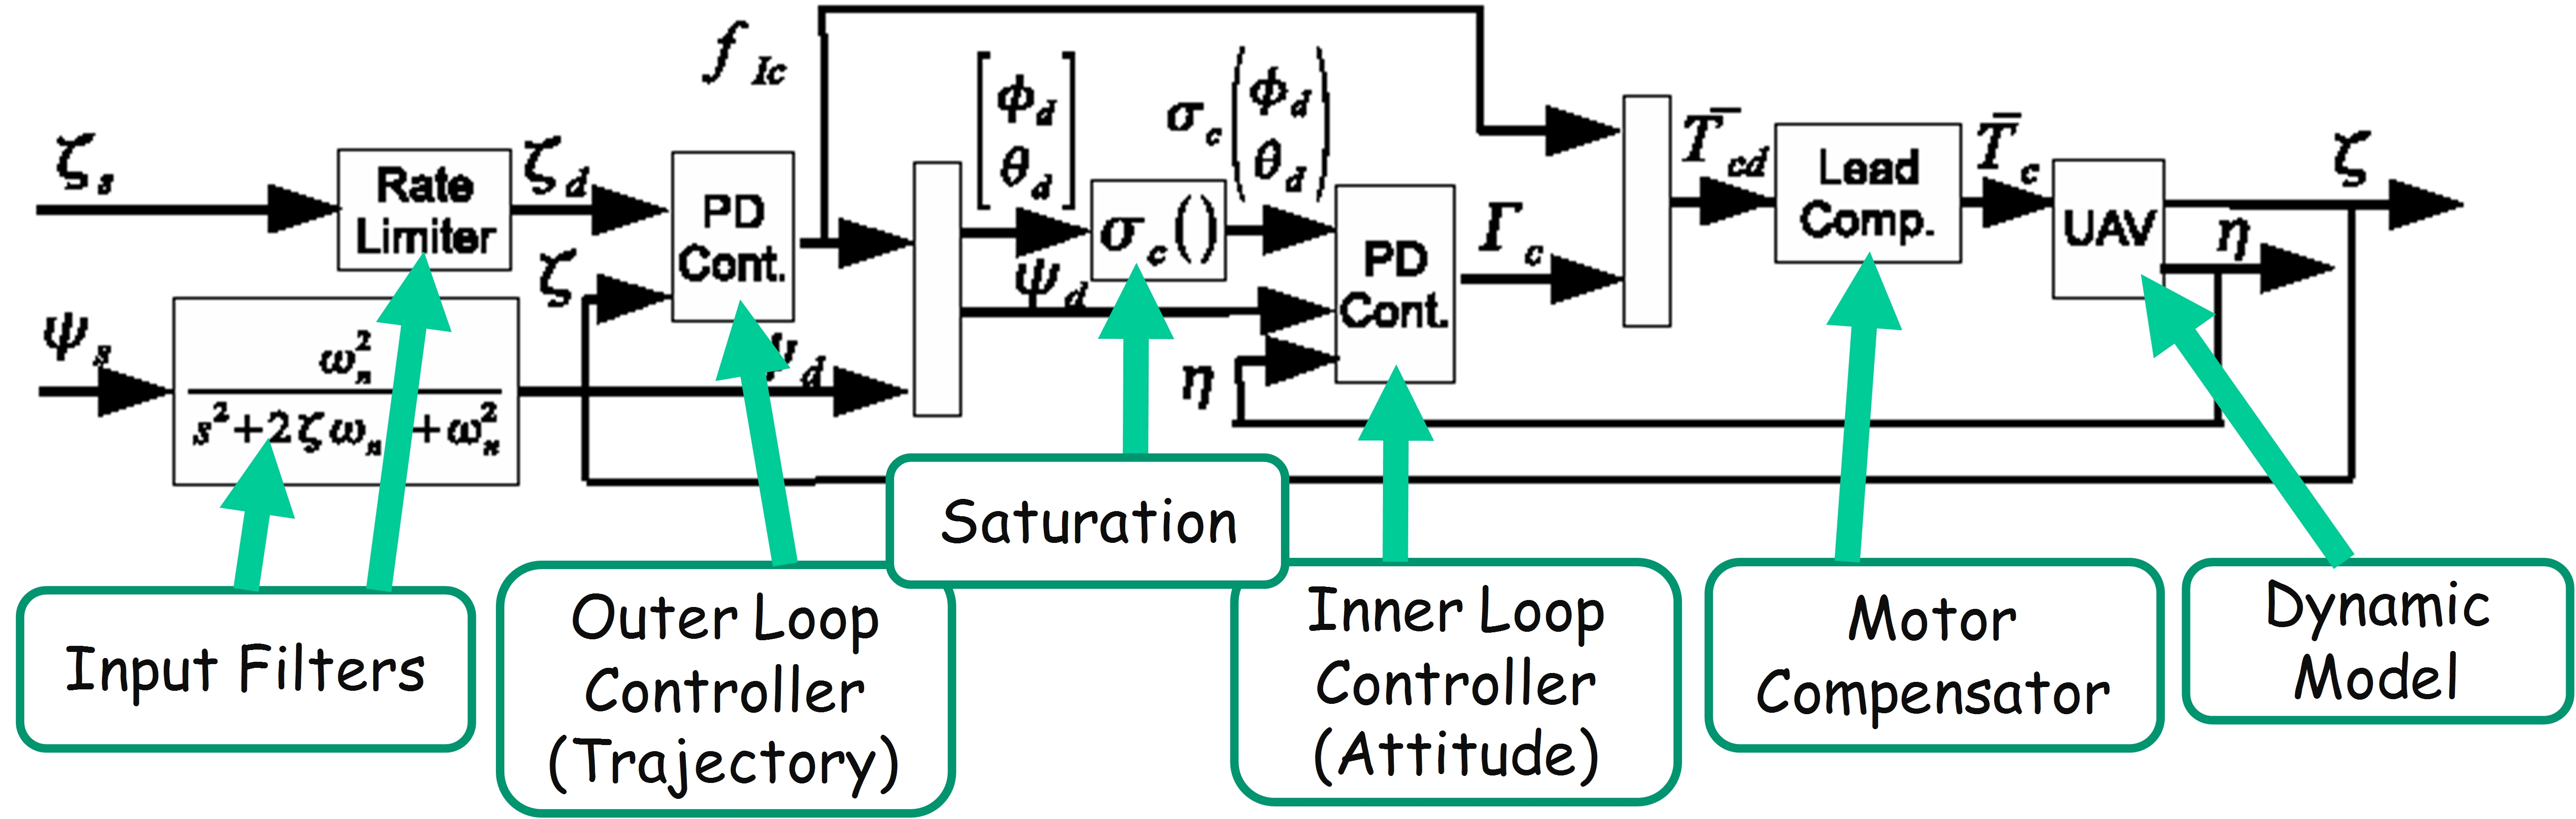
\includegraphics[width=\columnwidth]{figures/quadrotor_arch.png}
    \caption{Basic architecture for the quadrotor control problem.}
    \label{fig:quadrotor}
\end{figure}

Our design example controls a continuous-time system whose model represents a simplified 
version of a quadrotor UAV.  We exclude the nonlinear rotational dynamics of the actual 
quadrotor, but retain the stability characteristics.  For the fully detailed quadrotor model, 
see \cite{quad:passcontrol}.  The example model controls a stack of four integrators using 
two nested PD control loops, as shown in Fig. \ref{fig:quadrotor}.  The UAV block contains 
the integrator models. The two control loops (inner and outer, as shown) are implemented on 
separate processors, and the execution of the components is controlled by a simple time-triggered 
virtual machine that releases tasks and messages at pre-calculated time instants.

Control design centers around the continuous-time abstraction of passive control \cite{quad:passcontrol}.  
Passivity provides a robust version of continuous-time dynamic stability which is insensitive to 
quantization effects \cite{pass:fettweis86} and network delays \cite{ncs:chopra}\cite{ncs:wireless} 
in digital control implementations.  The passivity conditions help relax constraints on required 
component sample rates, increasing the system's tolerance to jitter and other timing variations.  
Note that control performance requirements could create additional constraints, but we do not 
address those here.  

Simulated stability analysis yields period parameters for the control components.  Here they 
represent nominal sample periods, but conservative parameters could also be represented.  For 
our discussion the exact nature of these parameters is not important, rather that they represent 
the same behaviors for all of the integrated tools.  Passive design provides a guarantee of stable 
operation around a nominal sampling rate, as the system will tolerate a small number of lost or 
delayed data samples.

\begin{figure}
\centering
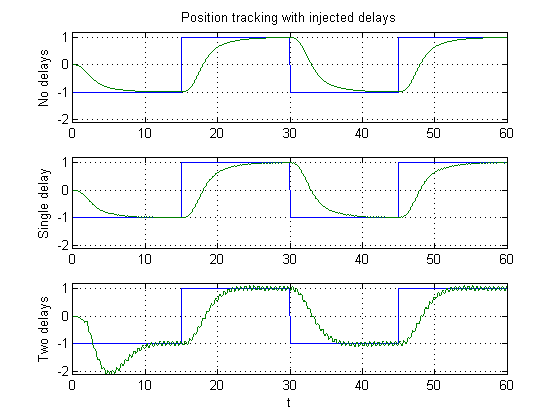
\includegraphics[width=0.9\columnwidth]{figures/delays.png}
    \caption{Effects of increasing delays in the synchronous scheduling of the control nodes.}
    \label{fig:delays}
\end{figure}


Our modeling tools include explicit platform and deployment modeling\cite{modeling:aces08}. 
Behavior of the deployed components depends on execution timing of the functions on the platform, 
the calculated schedule, and coordination between distributed tasks. The calculated execution schedule 
can be used to simulate the control design with additional delays to assess the impact of the platform 
on performance.  Fig. \ref{fig:delays} shows simulated effects of additional delays in the control data 
paths.  The top of the figure is the direct synchronous digital implementation of the control system.  
The two successive plots show the effects of adding first one and then two extra delay elements in each 
control path.  The reference input frequency and amplitudes were chosen to lie on the edge of the stable 
operating point of the design.  This is not meant to be an exhaustive verification of the control design, 
rather an illustration of the gradual oscillation and overshoot degradation that occurs as delays increase.  
See \cite{quad:passcontrol} for details of the design and its validation.

The passivity of the control components is an interface condition ($Power_{in} \leq Power_{out}$) that 
must be maintained in order to ensure the proper behavior of the design.  In the user language we select 
Simulink subsystems to be used as the specification of software components in the modeling language. Each 
will be implemented as a synchronous C function.  The selected component objects translate directly to 
component instances in the semantic language.  A component is an object with a unique name (i.e. InnerLoop), 
and information to find or generate its implementation in C (in this case, the filename and model path to 
the Simulink subsystem "`QuadIntegrator/InnerLoop"'). Though the robustness provided by the passive abstraction 
is not directly captured in our models (yet), it would be a more complex concept.  A useful abstraction of the 
behavior might be the maximum amount of tolerable time delay on each path (in synchronous time ticks) for the 
worst-case input for a particular control loop. Fig. \ref{fig:delay_abs} depicts a UML object diagram showing 
objects and relations in the abstract model that could represent such a concept.  The translation from a 
passive control component embedded in a design would have to visit all design model connections involved in the 
particular control interaction, and create the object and relations shown.  The first-stage model transformation 
would encode this structurally for all interpreters that make use of this bound object, ensuring that 
all of them work with the same semantic model.  Note that this is only a step in the right direction, as we 
have nothing yet in the language to ensure consistency at the level of equations that use these parameters.

\begin{figure}
\centering
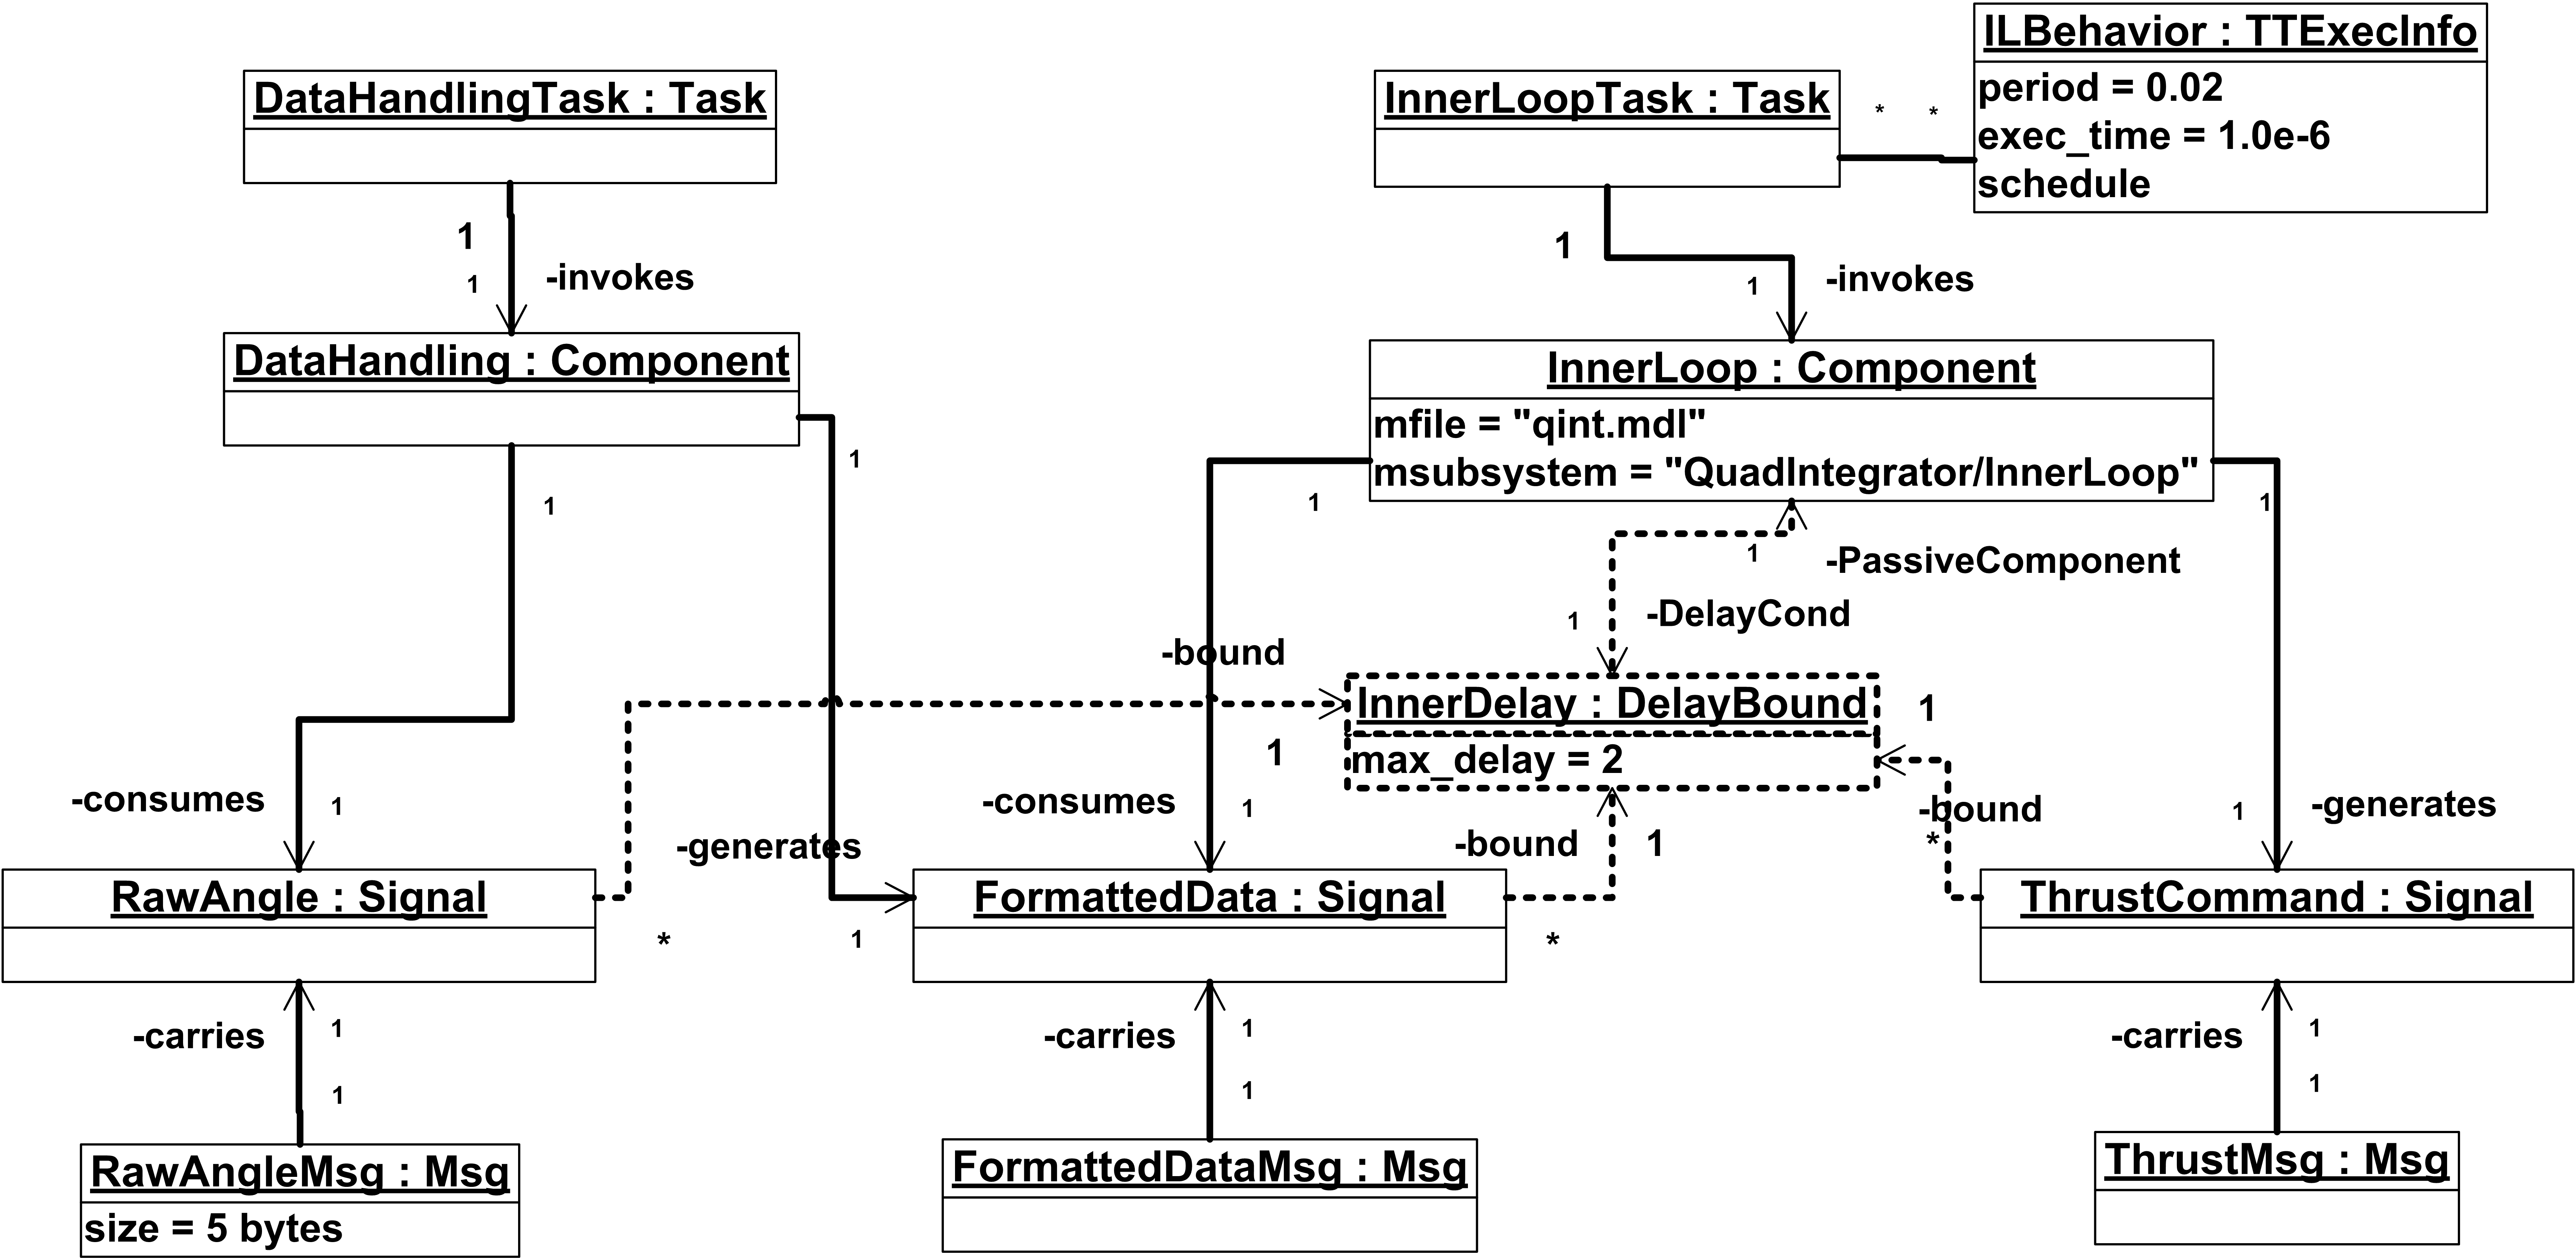
\includegraphics[width=\columnwidth]{figures/delay_bound.png}
    \caption{Capturing a delay bound in the semantic model.  The dashed object and connectors represent the 
concept to be represented. In practice each high-level design concept or bound is related to many other 
design object and their parameters.}
    \label{fig:delay_abs}
\end{figure}